%%%%%%%%%%%%%%%%%%%%%%%%%%%%%%%%%%%%%%%%%
% FRI Data Science_report LaTeX Template
% Version 1.0 (28/1/2020)
% 
% Jure Demšar (jure.demsar@fri.uni-lj.si)
%
% Based on MicromouseSymp article template by:
% Mathias Legrand (legrand.mathias@gmail.com) 
% With extensive modifications by:
% Antonio Valente (antonio.luis.valente@gmail.com)
%
% License:
% CC BY-NC-SA 3.0 (http://creativecommons.org/licenses/by-nc-sa/3.0/)
%
%%%%%%%%%%%%%%%%%%%%%%%%%%%%%%%%%%%%%%%%%


%----------------------------------------------------------------------------------------
%	PACKAGES AND OTHER DOCUMENT CONFIGURATIONS
%----------------------------------------------------------------------------------------
\documentclass[fleqn,moreauthors,10pt]{ds_report}
\usepackage[english]{babel}

\graphicspath{{fig/}}




%----------------------------------------------------------------------------------------
%	ARTICLE INFORMATION
%----------------------------------------------------------------------------------------

% Header
\JournalInfo{FRI Natural language processing course 2024}

% Interim or final report
\Archive{Project report} 
%\Archive{Final report} 

% Article title
\PaperTitle{Natural language processing course} 

% Authors (student competitors) and their info
\Authors{Veronika Durn and Ela Novak}

% Advisors
\affiliation{\textit{Advisors: Aleš Žagar}}

% Keywords
\Keywords{NLP, NLI, LLM, dialects, Slovenian language}
\newcommand{\keywordname}{Keywords}


%----------------------------------------------------------------------------------------
%	ABSTRACT
%----------------------------------------------------------------------------------------

\Abstract{
    This project explores Slovenian dialect exploration within the context of creating a Natural Language Inference (NLI) dataset. Our result is a dataset that challenges the comprehension abilities of Large Language Models (LLMs) regarding entailment, neutrality, and contradiction within longer text passages. Additionally, we focused on investigating the capacity of LLMs to accurately replicate various Slovenian dialects, including the Styrian dialect (štajersko narečje) and the Littoral dialect (notranjsko narečje). Through this exploration, we aimed to deepen our understanding of dialectical nuances and their implications for natural language processing tasks.

    Since this project focuses on researching Slovenian language and its dialects, a certain degree of proficiency in the language is required to make use of the findings.
}

%----------------------------------------------------------------------------------------

\begin{document}

% Makes all text pages the same height
\flushbottom 

% Print the title and abstract box
\maketitle 

% Removes page numbering from the first page
\thispagestyle{empty} 

%----------------------------------------------------------------------------------------
%	ARTICLE CONTENTS
%----------------------------------------------------------------------------------------

\section*{Introduction}

    This project aims to explore Slovenian dialects within the context of creating a Natural Language Inference (NLI) dataset. Our primary goal was to develop a dataset that challenges the comprehension abilities of Large Language Models (LLMs) regarding entailment, neutrality, and contradiction within longer text passages. Additionally, we focused on investigating the capacity of LLMs to accurately replicate various Slovenian dialects, including the Styrian dialect (štajersko narečje) and the Littoral dialect (notranjsko narečje). Through this exploration, we aimed to deepen our understanding of dialectical nuances and their implications for natural language processing tasks.

    Since this project focuses on researching Slovenian language and its dialects, a certain degree of proficiency in the language is required to make use of the findings.

%------------------------------------------------

\section{Theoretical background}

\subsection{Slovenian dialects}

    In Slovenia, one can find many different dialects, which exemplify the diversity and richness of  Slovene language and culture. In this study, we will examine two specific Slovene dialects, the Littoral dialect (notranjsko narečje) and the Syrian dialect (štajersko narečje), and assess how successfully certain Large Language Models replicate them.
    
    Understanding and documenting dialects is important for various reasons. It helps us to preserve the language and culture, and it is valuable resource for academia and research. By studying these dialects, our aim is to learn more about Slovenia's unique linguistic heritage and find metodologies for its  documentation in future research. 

    There are more than 30 dialects in Slovenia and they are divided into seven main dialect groups: the Littoral dialect group (\textit{primorska narečna skupina}), the Rovte dialect group (\textit{rovtarska narečna skupina}), the Upper Carniolan dialect group (\textit{gorenjska narečna skupina}), the Carinthian dialect group (\textit{koroška narečna skupina}), the Lower Carniolan dialect group (dolenjska narečna skupina), the Styrian dialect group (\textit{štajerska narečna skupina}), and the Panonian dialect group (\textit{panonska narečna skupina}). Some dialects are further divided into sub-dialects, and these, in turn, into different local speech varieties 
(Novljan, 2017). 

    However, it is important to note that the boundaries between dialects in Slovenia are not clearly defined, and even linguists disagree on the exact number of dialects. Some linguists even claim that there are between 40 and 50 different dialects. The variation in determining the precise number arises from significant differences between dialects, where speech patterns can vary even from one village to another. 

    \begin{figure}
        \centering
        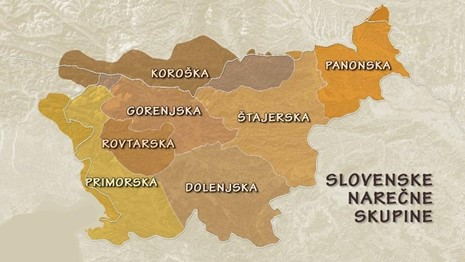
\includegraphics[width=1\linewidth]{narecne_skupine.jpg}
        \caption{Image 1: Slovene dialect groups
}
        \label{fig:map}
    \end{figure}

\subsubsection{Littoral Dialect Group}

    The Littoral dialect group comprises nine dialects: the Resian dialect (rezijansko narečje), the Torre Valley dialect (\textit{tersko narečje}), the Soča dialect (obsoško narečje), the Natisone Valley dialect (\textit{nadiško narečje}), the Brda dialect (\textit{briško narečje}), the Karst dialect (\textit{kraško narečje}), the Istrian dialect (istrsko narečje), the Čičarija dialect (\textit{čiško narečje}), and the Inner Carniolan dialect (\textit{notranjsko narečje}) (Novljan, 2017).

\begin{figure}
    \centering
    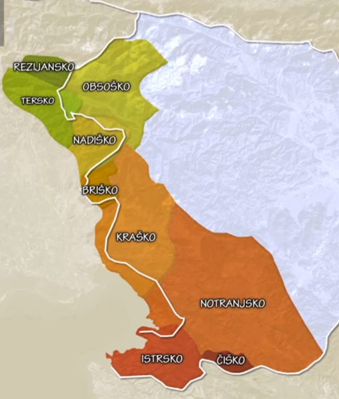
\includegraphics[width=0.5\linewidth]{Littoral.png}
    \caption{Image 2: Littoral dialect group
}
    \label{fig:map}
\end{figure}


\subsubsection{Styrian Dialect Group}

    The Styrian dialect group is spoken in the central and western parts of Slovenian Styria, in Maribor and its surroundings, in southern Pohorje, in lower and upper parts of Savinjska Valley, in Celje, Velenje, and the surrounding areas, as well as in Kozjansko and Bizeljsko. To the east, the Styrian dialect group extends to Slovenske Gorice and the lower course of the Drava river, gradually transitioning into the Panonian dialect group (Wikipedia, 2023).

    The Styrian dialect group is one of the seven main dialect groups in Slovenia and includes the following dialects: Central Savinja dialect (\textit{srednjesavinjsko narečje}), Upper Savinja dialect (\textit{zgornjesavinjsko narečje}) with Solčava sub-dialect (\textit{solčavsko podnarečje}), Central Styrian dialect (\textit{srednještajersko narečje}), Kozje-Bizeljsko dialect (\textit{kozjansko-bizeljsko narečje}), South Pohorje dialect (južnopohorsko narečje) with Kozjak subdialect (\textit{kozjaško podnarečje}), Lower Sava Valley dialect (\textit{posavsko narečje}) with Zagorje-Trbovlje subdialect (zagorsko-trboveljsko podnarečje), Laško subdialect (\textit{laško podnarečje}), and Sevnica-Krško subdialect (\textit{sevniško-krško podnarečje}) (Novljan, 2017). 
    
\begin{figure}
    \centering
    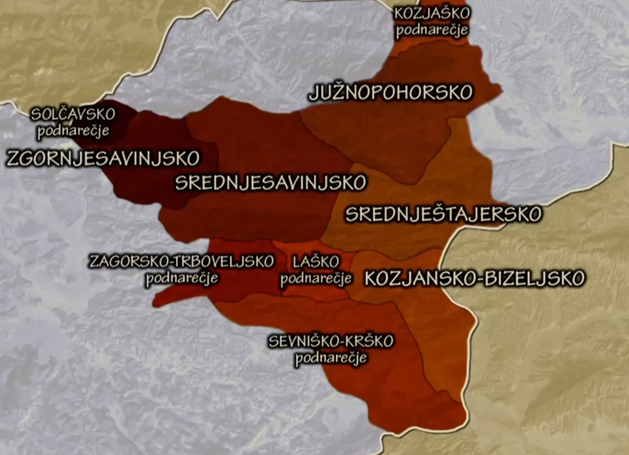
\includegraphics[width=1\linewidth]{styria.png}
    \caption{Image 4: Styrian dialect group
}
    \label{fig:map}
\end{figure}


    The Styrian dialect group also has some recognizable characteristics that distinguish it from other dialect groups: 

\begin{enumerate}
    \item The long stressed \textit{/e/} and falling \textit{/o/} developed into diphthongs \textit{/ei/} and \textit{/ou/}, while the old acute \textit{jat} was represented by the short narrow \textit{/e/}, and the new acute \textit{/o/} by the short \textit{/o/} (zvéizda, snéig, leis; mouč).

    \item The Upper Savinja dialect and Pohorje dialect are characterised by the lengthening of accented vowels, which is reflected in the double long representatives for \textit{/e/} and \textit{/o/} (zvâizda, snâik, pâič, brîza, nîsu in the Upper Savinja dialect and nusim, hudim in Pohorje dialect). 

    \item In some parts, the vowel \textit{/u/} changed to \textit{/ü/}, while in other parts remained the same or developed into \textit{/uu/} or \textit{/ou/}. The first change \textit{/ü/} is mainly found in the Central Styrian dialect. The vowel remained the same in the Central Savinja dialect and the Upper Savinja dialect. In the Pohorje dialect the vowel u developed into /\textit{uu/} or \textit{/ou/} (muha; müha; mu˛uha; mo˛uha).

    \item The long \textit{/a/} has been preserved in some parts of the Stryia territory, while in other parts it has been labiovelarized to a more or less wide \textit{/o/} (mačka; močka).

    \item The Styrian dialect does not distinguish between rising and falling accents in either long or short syllables. The tonal pattern in the Styrian dialect is mainly falling (Logar, 1975).
\end{enumerate}

\subsection{Natural language interference}
Natural language inference (NLI), also called textual inference recognition, is a task studied heavily in natural language processing. It helps with complex tasks like answering questions and summarizing text (Dagan et al., 2006). The main aim is to see if one sentence (the premise, p) implies another (the hypothesis, h) or not.

In a typical natural language formulation of a logical inference problem, two sentences are entered. The first is called the premise, the second the hypothesis. If the hypothesis is a logical consequence of the premise, or if we can reasonably infer the truth of the hypothesis on the assumption that the premise is true, we call this relationship entailment. If the information in the hypothesis contradicts that in the premise, or if we can reasonably infer the falsity of the hypothesis from the truth of the premise, we call this a contradiction. If, on the other hand, we can conclude neither the truth nor the falsity of the premise from the premise, i.e. if the information in the premise neither confirms nor rejects the hypothesis, this is the case of neutrality. This is essentially a classification problem, but it can be extended to require explanations in addition to classification. The fact that the language model that solves the problem must justify the answer gives us further insight into its approach to solving the problem (Bowman et al., 2015).  


%------------------------------------------------

\section{Methodology}

\subsection{Selection of Large Language Models}

    In the initial phase of our research, we evaluated the available Large Language Models (LLMs) that are suitable for our project's aim. After a thorough assessment, we decided to use the open-source language models Gemini and GPT-3.5. These selections were based on their demonstrated proficiency in understanding and modeling the Slovenian language.

    Within our methodology, we also examined alternative LLMs such as Llama 2 and Llama 3 to assess their suitability for replicating Slovenian dialects. However, these models proved to be insufficiently trained on Slovenian texts, which impaired their ability to successfully imitate the language, let alone its dialects.
    
\subsection{Prompts design}

    To ensure the accurate representation of Slovenian dialect nuances, we carefully created 25 prompts tailored to each dialect. These 50 prompts (25 for each dialect) were designed to incorporate dialect-specific vocabulary, grammatical structures, and cultural references, facilitating the understanding and reproduction of dialectal variations by the Large Language Models (LLMs). 
    
    To ensure robustness and generalisability of our results, we incorporated a wide range of topics and genres into our prompts. These prompts ranged from everyday conversations to technical discussions, literary extracts, and cultural and historical references, providing a diverse testing ground for the LLMs' dialectical reproduction abilities. By exposing the models to different linguistic contexts, we aimed to capture their performance in different fields and settings.
    
\subsection{Execution and response retrieval}

    After designing the prompts, we inputted them into the selected LLMs, comprising of Gemini and GPT-3.5, using their respective APIs or interfaces. Once the prompts were entered, we waited for the models' responses, which were autonomously generated  based on the provided instructions and the models' learnt patterns and language understanding capabilities.
    
\subsection{Data collection and analysis}

    After the prompts were executed, we systematically documented the responses generated by the LLMs in separate documents. Each document contained the LLM's responses to the prompts in the two different dialects, enabling the capture of nuanced linguistic variations produced by the models. This documentation process ensured the preservation and organisation of the response data for further analysis.

    For a comprehensive analysis, we created a separate set of documents for each LLM and each dialect. This approach allowed us to compare how well each specific model replicated dialects in general versus how the models in general replicated a specific dialect. By splitting the response data into separate sets of documents, we were able to isolate and evaluate the performance of each LLM across different dialectal variants more efficiently.

    With the document sets established, we conducted a comparative analysis to evaluate the accuracy of dialectal reproduction produced by each LLM. This analysis involved examining lexical choices, grammatical structures, idiomatic expressions, and cultural references within the generated responses. By comparing the responses between the different dialects and models, we were able to gain insights into the models' ability to reproduce dialectal nuances and their overall performance in dialect reproduction tasks.

\subsubsection{Natural Language Inference assesment }

    To determine the Natural Language Inference (NLI) labels for the models' responses, we established a framework that evaluated the responses according to two main factors. Firstly, we checked whether the responses aligned with the provided context and genre given in the instructions. Secondly, we analysed whether the dialect use matched the given prompt. The criteria for assigning NLI labels were as follows:

1. \textbf{Entailment}: This label is assigned when the generated response follows the instructions regarding context and the number of paragraphs (each paragraph has around 5 sentences). The dialect is also present throughout the whole text.

2. \textbf{Neutral}: This label is assigned when the generated response follows the instructions for context and paragraph length, where each paragraph contains somewhere between 3 and 7 sentences, and/or when the dialect is present but not throughout the entire text. The model also uses standard Slovene and other dialect expressions, slang, jargon, etc.

3 \textbf{Contradiction:} This label is assigned when the response does not follow the instructions on the context and the number of paragraphs and sentences and/or when dialect is not present or is written entirely in standard Slovene or another dialect.

\subsection{Creation of a dataset}

After collecting and evaluating the data, we then began with a dataset creation. The dataset was created based on the 50 prompts. Each prompt was kept the same as it was presented to the LLMs, but the answers were changed. We manually wrote the answers according to the specified dialects (Styrian and Littoral dialects). This was possible due to each of us being native speakers of one of the dialects.

\vspace{\baselineskip}
Examples of dataset paragraphs are:
\vspace{\baselineskip}

\textbf{1. Littoral dialect}

\textbf{Prompt}: Napiši besedilo dolgo 2 odstavka. Vsak odstavek naj ima približno pet povedi. V prvem odstavku piši o začetkih čevljarstva v kraju Miren, v drugem odstavku pa piši o o podjetju Ciciban. Da bo besedilo bolj avtentično, ga napiši v izrazitem notranjskem narečju.

\textbf{Response}:
\textit{Mjrn ima dowgoletno čewljarsko tradiciju in j znan po eni prvih čevljarskih zadrug pr ns. Že pred prvu svetowno vojnu se j v zadrugu povjzlo 18 čewljarskih mojstrow in skorej stu njihovih vajencu. Kdr se j zčjla vojna, so izdelavli škwrne z vojake, k so jih pwol z ulaki rznašli na wkrwh. Dns u Mjrni stoji tudi čewljarski muzej, k ga j dau uredit Pavel Peteljan, k velja z enga wd zčetniku wtrwške obutve Ciciban. 
Zgodovina Cicibana j povjzna s čewlarjm Tomažm Vukm, k je ljta 1952 rzstavu vzorce wtrwškega obuvala, k ga j poimenovau Ciciban. Ivan Petejan je pwol svojo obrt predau sinu, k je ndljevau tu čewljarsku tradicijo in počasi j podjtje ratlo znanu po cjli Sloveniji, Istri in še Dalmaciji. Podtjeje še dns deluje in trude ohranjt stare čewljarske veščine. Usi čjwli so rwočno nrjeni, kar jim daje posjbno vrednost. Podjtje je ponos Slovenije in prnaša prepoznavnost cjli regiji. }

 
\vspace{\baselineskip}
\textbf{2. Styrian dialect}

\textbf{Prompt:} Napiši besedilo o nočnem nebu in ozvezdjih. Besedilo naj bo dolgo 2 odstavka. Vsak odstavek naj ima približno pet povedi. V prvem odstavku se osredotoči na zvezde na splošno, v drugem pa na različna ozvezdja. Da bo bolj avtentično, besedilo napiši v izrazitem štajerskem narečju. 

\textbf{Response:}
\textit{V toto našo nebo so že od nekdaj zijali ludi pa se spraševali ka pomenijo zvezde pa to. Ko zvezde so res taka zanimiva zadeva, ko fčasih sploh nena morš verjet kak daleč so pa zaka jih sploh vijiš ponoči. Pa včasih se ti zdi da ftriplejo, pa so te še bol zanimive. Pol pa či pomisliš je dejansko fsaka zvezda tako našo sonce pa ma okoli solarni sistem, to je tak težko razumet, kolko planetov sploh obstaja.}
\textit{Či pa dolgo v njih buliš pa se ti lahko začnejo prikazovat ozvezdja, ko se ti zdi da so med samo povezane zvezde pa iz jih nastane neka oblika, ko si jo fsak drugače predstavla. Tou so ludi že od nekdaj dejlali, te pa so se nekak ustalila imena totih ozvezdij, da jih še gnes uporablamo ko jih glejamo.}

\subsection{Insertion of dataset into an LLM and training}

After compiling the dataset, we then inserted it into the LLM, which we evaluated as generating better responses. In our case, this was the GPT-3.5 model. We presented the dataset as a prompt to the model and trained it accordingly to the dialect.

\subsection{Re-generation and evaluation of responses}

Once the dataset was successfully integrated in the language model, we asked it to once again generate the responses to the same prompts and compared them to the original responses. Our results can be found in the \textbf{Results after manual written dataset} section of the paper.


 

%------------------------------------------------

\section{Evaluation of LLMs}

    In this chapter, we will delineate a series of methodological challenges encountered while formulating prompts for Gemini and GPT-3.5.

\subsection{Gemini}

    During our exploration of text generation with Gemini, we encountered a series of methodological challenges. Our analysis revealed that Gemini often produced more paragraphs than instructed, despite explicit directives to produce only two paragraphs. Furthermore, it frequently disregarded the instruction specifying that each paragraph should consist of a maximum of five sentences. Clarity regarding paragraph and sentence structure was in some examples achieved only when explicit instructions were provided - to generate precisely two paragraphs, each with a maximum of five sentences. Although the prompts did not explicitly call for the inclusion of a title and conclusion, Gemini, in most instances, produced titles for both the first and second paragraphs and concluded with a final thought on the text. 

    However, a more significant issue occurred when we attempted to generate dialect-specific content. Despite instructions to produce distinctly dialectal content, Gemini predominantly produced a text in standard Slovene. Despite additional prompts, Gemini still predominantly produced texts in standard Slovene and included numerous linguistic fillers (such as \textit{pač}), interjections (such as \textit{joj}), rhetorical figures (such as \textit{slikoviti griči}, \textit{ponosni stražarji}, and \textit{sonce na krožniku}), rhetorical questions (such as \textit{Družina, ja to je pa nekakšen temelj našega življenja, mar ne?}), and colloquial expressions (such as \textit{ful}, and \textit{faca}), rather than incorporating authentic dialectal expressions. It was only upon repeated prompts that Gemini exhibited some degree of dialectal authenticity, which was predominantly present in the first paragraphs of the texts.  

\subsection{GPT-3.5}

While working with OpenAI’s large language model GPT-3.5, we noticed the following:

    Firstly the model adhered well to the context-based instructions regarding the topic of the text and its length. It never generated a response that was too short or long and it stuck to the instructed topic. 

    Secondly, the model often produced passages in standard Slovene (knjižna/standardna slovenščina). This most often occurred in the model’s first response to the prompt. It almost seemed as if the model ignored the instructions to write in the specified dialect (either the Styrian or Littoral dialects). However, when another prompt followed with the instructions to once again “remind” the model to produce text that is not standard, GPT-3.5 managed to include regional and dialectal words, phrases, and other linguistic elements. 

An example of such behaviour is:
\vspace{\baselineskip}

\textbf{Prompt}:
Napiši besedilo o tem, kako tehnologija vpliva na ljudi. Besedilo naj bo dolgo 2 odstavka, v prvem se osredotoči na vpliv po vsem svetu, v drugem pa na Slovenijo. Da bo bolj avtentično, ga napiši v izrazitem štajerskem narečju.

\textbf{Answer:}
\textit{Tehnologija je postala nepogrešljiv del našega vsakdana in vpliva na nas na mnogo načinov po vsem svetu. Z razvojem pametnih telefonov, računalnikov in družbenih omrežij smo postali bolj povezani in informirani kot kdajkoli prej. Vendar pa lahko pretirana uporaba tehnologije vodi v izolacijo, pomanjkanje fizične aktivnosti ter težave s spanjem in duševnim zdravjem. Poleg tega tehnološki napredki prinašajo tudi nove izzive, kot so varovanje zasebnosti, kibernetski napadi in odvisnost od digitalnih naprav.}

\textit{V Sloveniji pa je vpliv tehnologije podoben kot drugod po svetu. Pametni telefoni, računalniki in internet so postali nepogrešljiv del vsakdana tudi tukaj. Ljudje se povezujejo preko družbenih omrežij, opravljajo nakupovanje preko spleta in izvajajo delo na daljavo. Vendar pa je pomembno, da se zavedamo pasti pretirane uporabe tehnologije in da znamo najti ravnotežje med digitalnim svetom in resničnim življenjem. Spremljanje novih tehnoloških trendov je pomembno tudi za slovensko družbo, saj lahko tehnološki napredki prinašajo tako priložnosti kot tudi izzive.}

\textbf{Follow-up prompt:}
Besedilo napiši bolj narečno - v štajerskem narečju.

\textbf{Follow-up answer:}
\textit{Tehnologija je že postala del našega vsakdana pa vpliva na nas na mnogo načinov po vsem svetu. Z razvojem pametnih telefonov, računalnikov pa družbenih omrežij smo postali bolj povezani pa informirani kak kdajkoli prej. Ampak, preveč ziher uporabe tehnologije pa lahko pelje v izolacijo, manko fizične aktivnosti pa težave s spanjem pa duševnim zdravjem. Pa tudi tehnološki napredki prinesejo nove izzive, kak so varovanje zasebnosti, kibernetski napadi pa odvisnost od digitalnih stvari.}

\textit{V Sloveniji pa je vpliv tehnologije podoben, kak drugje po svetu. Pametni telefoni, računalniki pa internet so že postali del vsakdana tut tle. Ljudje se povezujejo preko družbenih omrežij, opravljajo nakupovanje preko spleta pa delajo od doma. Ampak, pomembno je, da se zavedamo pasti preveč uporabe tehnologije pa da znamo najti ravnotežje med digitalnim svetom pa realnim življenjem. Spremljanje novih tehnoloških trendov je tudi tuki pomembno, ker tehnološki napredki lahko prinesejo tako priložnosti pa tudi izzive za slovensko družbo.}
\vspace{\baselineskip}

    After nudging the model to write more in-line with the mentioned dialect, one can also observe how it indeed wrote the passage with “strong” dialectal elements (in this case with words such as \textit{pa, kak, ziher, tut }etc.), but the way they fit into the text makes little sense to the native speaker of the dialect. Most of the passage is still in-line with standard Slovene and the regional nuances seem to be placed into the text at random. An example of this is the model keeping the standard word \textit{tudi }(‘also’) for most occurrences, but switching to its dialectal variant \textit{tut} only once. It would make “sense” for the model to switch either 100\% or 0\% of the time, but this was not the case.

    Another issue worth mentioning is how the model switched between dialects. When producing answers in a specific dialect, it often switched to another dialect at, what seemed, random. This can also be observed in the above example. The model used \textit{tle }and \textit{tuki} as variants of the standard Slovene \textit{tu/tukaj }(‘here’), but these words are not a part of the Styrian dialect, as they most commonly belong to the dialects found in more central Slovenia.



%------------------------------------------------

\section{Results}

When analyzing the Styrian dialect (štajersko narečje) and Littoral dialect (notranjsko narečje), we noticed great disparities between the two models. Due to the apparent differences, we will present our findings for each model and dialect separately.

\subsection{Littoral dialect}
\vspace{\baselineskip}
\subsubsection{GPT-3.5}

    When considering the instructions regarding the length and the genre of the text, the GPT-3.5 model consistently adhered to the guidelines and did not exceed the limitations regarding paragraphs and the number of sentences per paragraph. The generated paragraphs within texts were clearly connected, with paragraphs complementing each other, thus ensuring that all generated texts maintained a logical coherence. 

    Regarding adherence to instructions for generating text in the Littoral dialect (notranjsko narečje), GPT-3.5 was not as successful. Following the initial instructions, it predominantly produced texts in standard Slovene (standardna/knjižna slovenščina). After additional prompts and instructions, it yielded improved results, yet the texts still remained rich with expressions in standard Slovene. In some instances, it utilized expressions from the Lower Caroniolan dialect (such as \textit{tut}, \textit{važn}, \textit{dost} etc.) and incorporated numerous colloquial and slang expressions (such as \textit{ful}, \textit{fora}, \textit{fajn}, \textit{folk} etc.). In some texts it still produced some distinctly Littoral dialect expressions (such as \textit{kanta}, \textit{spoštavajo}, \textit{našga}, \textit{proba}, \textit{pr}', \textit{en caj}t etc.). However, at times, despite the instruction to write the text in the Littoral dialect, it incorporated expressions from other dialectal groups (such as \textit{kak}, \textit{tut}, \textit{ka} etc).

\vspace{\baselineskip}
Inference in numbers:
\n\\ \textbf{Entailment}: 0 (0\%)
\textbf{\n\\Neutral}: 23 (92\%)
\textbf{\n\\Contradiction}: 2 (8\%)

\vspace{\baselineskip}
Most results were therefore classified as neutral, with contradiction being second-most common result, and entailment appearing in zero cases.


\subsubsection{Gemini}

    In terms of adhering to the content and genre instructions, Gemini performed equally well as the GPT-3.5 model. However, regarding the length of the text, Gemini in most cases exceeded the specified limitations. It added more paragraphs, with paragraphs being longer than the specified limit, and frequently provided a conclusion at the end of the text. Another distinction is that Gemini generated titles for each paragraph, even though this was not specified in the instructions. 

    In generating text in distinctive Littoral dialect (notranjsko narečje), Gemini's performance was inferior to that of GPT-3.5. Initially, similar as GPT-3.5, it produced predominantly standard Slovene texts. However, with additional prompts and instructions, it gradually incorporated some Litteral dialect expressions (such as \textit{inu}, \textit{finte}, \textit{proba}, \textit{fešta}, \textit{bejž'te}, \textit{pr' }etc.). Throughout, it used numerous linguistic fillers (such as \textit{pač}, \textit{pa} etc.). Similarly to GPT-3.5, it utilized a lot of colloquial and slang terms (such as \textit{fajn}, \textit{faca}, \textit{fora} etc.). Unlike GPT-3.5, Gemini also incorporated some rhetorical figures (such as \textit{sonce na krožniku}, \textit{slikoviti griči} etc.) and some diminutives (like \textit{mestece}, \textit{cvičkotom} etc.). An important observation is that in the first paragraph generated more Littoral  dialectal expressions compared to the second paragraph. 

    \vspace{\baselineskip}
Inference in numbers:
\n\\ \textbf{Entailment}: 0 (0\%)
\textbf{\n\\Neutral}: 1 (4\%)
\textbf{\n\\Contradiction}: 24 (96\%)

\vspace{\baselineskip}
Almost all results were therefore classified as a contradiction, with one case of neutrality and no cases of entailment.
    
\subsection{Styrian dialect}
\vspace{\baselineskip}
\subsubsection{GPT-3.5}

    When it comes to context and genre, GPT-3.5 followed the requested topics 100\% of the time. It clearly had no trouble writing an answer that was contextually in-line with the prompt.

    However, it did not perform as well in regards to the dialect criteria. While it adhered to the Styrian dialect some of the time, its answers were most frequently classified as neutral. This is due to the fact that while it often produced some dialectal words and patterns, it also included some words from other dialects and/or in standard Slovene. It never received a contradiction label, as there was no case where it did not use at least some words in the specified dialect. 

    Another observation is the fact that, as mentioned above, it often did not produce a dialectal text from the first prompt. We sometimes had to give it a follow-up prompt in order for it to produce an answer that was not written in standard Slovene.
    
\vspace{\baselineskip}
Inference in numbers:
\n\\ \textbf{Entailment}: 3 (12\%)
\textbf{\n\\Neutral}: 12 (48\%)
\textbf{\n\\Contradiction}: 10 (40\%)

\vspace{\baselineskip}
Most results were therefore classified as neutral, with contradiction being second-most common result, and entailment being the rarest.

\subsubsection{Gemini}

    Context- and genre-wise, Gemini performed just as well as GPT-3.5. Like GPT-3.5, the model had no issues with generating text that followed the topic provided in the instructions. As mentioned above, it did, however, have great difficulties with following the paragraph length limit.

    When it comes to dialects, the results were much worse than GPT-3.5. It failed to receive a single entailment tag. This is mostly due to the facts mentioned above, namely that it almost always produced text in standard Slovene. It sometimes began the excerpt with a single sentence that contained a few Styrian dialectal words, but then went on to write everything else in standard Slovene.
    
\vspace{\baselineskip}
Inference in numbers:
\n\\ \textbf{Entailment}: 0 (0\%)
\textbf{\n\\Neutral}: 2 (8\%)
\textbf{\n\\Contradiction}: 23 (92\%)

\vspace{\baselineskip}
Most results were therefore classified as a contradiction, with neutrality being second-most common result (however, appearing only two times), and entailment appearing zero times.


%------------------------------------------------
\section{Results after manual written dataset}

We each created 25 manually written texts, aiming to closely resemble the natural speech of speakers of  Littoral and Styrian dialects. Once we compiled all the texts, we inputted this dataset into GPT-3.5 due its superior performance compared to the Gemini model. Initially, we provided GPT-3.5 with the first half of the dataset, followed by the second half due to its word limits. Overall, we observed an improvement in results. Notably, in certain cases, it produced dialectical texts of exceptional quality, closely aligning with the speech of native speakers of these dialects. These appeared mostly in the Littoral dialect, as the differences in generated texts before and after inputting the dataset were not as starkly apparent in the Styrian dialect.

We also observed that from the dataset we provided, GPT-3.5 compiled a list of rules for the Styrian and Littoral dialect. In addition, we noticed that GPT-3.5 needed to be prompted several times to properly utilize the knowledge acquired from the data set. Overall,  we observed disparities between the two dialects. Due to the apparent differences, we will present our findings for each dialect separately.

\vspace{\baselineskip}
\subsection{Littoral dialect}

During the comparison of result before and after the inserted data into GPT-3.5, we noticed several significant differences worth highlighting. 

Prior to providing GPT-3.5 with the dataset necessary for learning the correct generation of the Littoral dialect, the model generated 23 texts that corresponded to neutrality  and 2 text that corresponded to contradiction. After inputting the dataset, there was a notable improvement in the outcome, as the model produced 10 generated texts that were in line with entailment. However, 13 generated texts remained neutral and only 2 texts correlated with contradiction. It is important to note that only in one case (prompt 13), GPT-3.5 generated poorer quality text compared to before. 

    \vspace{\baselineskip}
Inference in numbers after the dataset:
\n\\ \textbf{Entailment}: 10 (40\%)
\textbf{\n\\Neutral}: 13 (52\%)
\textbf{\n\\Contradiction}: 2 (8\%)

\vspace{\baselineskip}

Secondly, it is important to highlight that during the process of learning from the dataset, the model compiled a list of rules and characteristics specific for Littoral dialect. The rules that it managed to extract are presented below. 

\begin{enumerate}
    \item spelling and pronunciation:
    \begin{itemize}
        \item replacement of "i" with "j" (e.g., "zjutraj" becomes "zwdej")
        \item replacement of "v" with "u" or "w" (e.g., "voda" becomes "woda")
        \item omission or replacement of vowels (e.g.,  "ljudi becomes "ldje")
        \item use of conjunction "j" instead of "je" (e.g., "j bogati")


    \end{itemize}
    \item Sentence structure:
    \begin{itemize}
        \item simpler sentence structure with shorter sentences
    \end{itemize}
\item Specific words and phrases:
\begin{itemize}
    \item  "tako"  becomes "tku"
    \item "dobro" becomes "dwobro"
    \item "zelo" becomes "zlu"
    \item "živali" becomes "žvali"
    \item "ljudi" becomes "ldje"
    \item "otroci" becomes "wtroci"
    \item "tradicija" becomes "tradiciju"
    \item "res" becomes "rjs"
    \item "pač" becomes "pej"
    \item "ko" becomes "kdr"
\end{itemize}
\end{enumerate}

Lastly, we would like to highlight one example that meet the criteria of entailment after the inputted dataset to prove the improvement of GPT-3.5 after training. The instruction was to generate a text discussing the history of the Eurovision in the first paragraph and Slovenian representatives who participated in the Eurovision in the second paragraph. 

\vspace{\baselineskip}
The generated text: 

\textit{Evrovizija je začela l. 1956 k mali tekmvanje, zdej pa j postala en najblj znanih śowow u svejtu. Z vsako leto se zbere dwosti držav, k tekmujejo z dwobro muzko pa pesmami. Vsaka država pošle swojga predstavnika, k pol poje n wejkmi śowu, k se predvaja pwsod. Tekmvanje je znano po barvitih nastopih, zanimivih kostumih in raznolikih žanrih. Pwsod prwlači velik gledalcev, k podpirajo swoje favorite pa uživajo u spektaklu.}

\textit{Slovenija je prvič sodelovala na Evroviziji l. 1993, k smo pošlali 1x svojo pesem. Ena najblj znanih predstavnic je bila Rebeka Dremelj s pesmijo "Vrag naj vzame" l. 2008. Tud Maraaya sta dosegla dwosti pzornosti s svojo pesmijo "Here for You" l. 2015. Pa še polk ne pozabmo na slovenko Darjo Švajger, k je dvakrat nastopila in dosegla dwobro uvrstitev. Naši predstavniki se trudjo pokazat swoj talent pa predstavt Slovenijo na najbolši možn način.}

\vspace{\baselineskip}
In this text, GPT-3.5 appropriately adhered to the rules and characteristics of Littoral dialect. The conjunction "je" was correctly replaced with the simplified conjunction "j", vowels were appropriately ommited in certain words (e.g., "najbl" instead of "najbolj, "muzko" instead of "muzika"), in some words "v" was replaced with "w" (e.g., "dwobro" instead of "dobro", "pwsod" instead of "povsod", "prwlači" instead of "privlači", "swoje" instead of "svoje", etc.). The conjunction "ki" was also correctly replaced with simplifed conjunction "k". 

Although GPT-3.5 generated significantly improved texts after the dataset input, as demonstrated in the text above, it required substantial prompting and remainders to adhere to the dataset that was provided. 


\subsection{Styrian dialect}

When comparing results before the insertion of the dataset and after it, there are a few things worth noting when it comes specifically to the Styrian dialect as well.

Firstly, the GPT-3.5 model compiled more answers we evaluated as entailment than before. In numbers, there were 11 cases of entailment, 9 cases of neutrality, and 5 cases of contradiction, as opposed to previous results, where there were  3 cases of entailment, 12 cases of neutrality, and 10 cases of contradiction. According to these results, it can be implied that the results were significantly better after the introduction of the dataset. 
    
\vspace{\baselineskip}
Inference in numbers after the dataset:
\n\\ \textbf{Entailment}: 11 (44\%)
\textbf{\n\\Neutral}: 9 (36\%)
\textbf{\n\\Contradiction}: 5 (20\%)

\vspace{\baselineskip}
Most results were therefore classified as an entailment, with neutral being second-most common result, and contradiction being the rarest.

Secondly, the positive change was not always the case, as the second text generation sometimes produced worse results than the first generation without the dataset (e.g. being classified as a contradiction, whereas the previous answer was classified as neutral). However, there were significantly fewer such cases compared to the opposite scenario of the second generation scoring higher.

It is also worth noting that in the second text generation, the model occasionally produced answers that were not in-line with instructions in terms of paragraph structure. It seemed that when emphasizing that the model adhere to the Styrian dialect, it ignored the instructions about the text structure and length. This was especially interesting, as GPT-3.5 did not have any issues with following such instructions the first time we asked it to generate passages (before introducing the dataset).

The model also identified certain "rules" when learning from the dataset. They are presented below.

\begin{enumerate}
    \item Phonetics and pronunciation: 
        \begin{itemize}
        \item some characteristic phonetic features are observed, such as the use of "f" instead of "v" in words ("fčasih" instead of "včasih")
        \item use of "kuj" instead of "zdaj"
        \item there are also characteristic accent patterns that differ from standard Slovene
    \end{itemize}
    \item Vocabulary:
        \begin{itemize}
        \item some terms and words may differ from standard Slovene
        \item use of "toti" instead of "ta"
        \item use of "fčasih" instead of "včasih"
        \item use of "tuji" instead of "tako", etc
    \end{itemize}
    \item Verbs and phrases:
        \begin{itemize}
        \item the use of verbs and phrases can reflect local idiosyncrasies
        \item use of "špilat" instead of "igrati"
        \item use of "prčkarije" instead of "mali popravki", etc.
    \end{itemize}
    \item Syntactic structure:
        \begin{itemize}
        \item the syntactic structure of sentences may vary
        \item use of phrases such as "pa tak" or "zaj ka"
    \end{itemize}
    \item Regional and cultural features:
        \begin{itemize}
        \item the texts also include descriptions of local places, customs and traditions, which are typical of the Styria region
    \end{itemize}
\end{enumerate}

 Lastly, when comparing the results of the generated responses in the Styrian dialect to those in the Littoral dialect, one can observe that there was no instance where the model was able to "almost perfectly" replicate the Styrian dialect, whereas there were cases in the Littoral dialect where this was present.


%------------------------------------------------
\vspace{\baselineskip}
\section{Discussion}
In this section, we will focus on the possible implications of the results, as well as evaluate what could be done to provide better results.

\subsection{Result implications}
Our results showed that the input of a dataset into the GPT-3.5 large language model had beneficial results in terms of determining natural language inference scores. Both dialects scored higher after the LLM training. 

These results indicate that GPT-3.5 can effectively improve natural language understanding in different dialects. The improvement in results after training suggests that the model is able to adapt well to different linguistic prompts, which is crucial for applications that require robust language understanding. This is consistent with previous studies in which large language models showed significant improvements in various NLP tasks after fine-tuning with relevant datasets (Brown et al., 2020; Raffel et al., 2020).

In addition, the increase in scores in both dialects emphasises the model's ability to help close gaps in language variation. This is particularly important for the development of language technologies that cover a wide range of speech communities, ensuring inclusion and reducing bias. Our results support the hypothesis that large language models can help to achieve more uniform performance across different language varieties (Bender et al., 2021).

However, it is important to recognise the limitations of our study. While the improvement in natural language reasoning results is promising, the extent to which these improvements can be transferred to real-world implementations remains to be explored in depth. Future work should investigate the performance of the model in more complex and diverse linguistic contexts to ensure its reliability and robustness in practical scenarios.

 

\subsection{Possible solutions}

    When analyzing the produced texts and our prompts, we came up with a few solutions that could help the models get better scores according to NLI tagging. We present the solutions in the following subsections.

\subsubsection{Follow-up prompts with dialect emphasis}

    An effective solution we implemented to improve the accuracy of dialectal reproduction by the LLMs was the use of follow-up prompts emphasising the use of the target dialect. After receiving the initial responses from the language models, we developed follow-up prompts that reiterated the previous instructions while explicitly emphasising the specific dialect that the model was to reproduce. By reinforcing the dialect and providing clear instructions, these follow-up prompts served to guide the LLMs towards more accurate and authentic dialectal responses.

\vspace{\baselineskip}
An example of this can be observed in the following prompt that was conducted on GPT-3.5:

\vspace{\baselineskip}
\textbf{Prompt}: 
Napiši besedilo dolgo 2 odstavka. Vsak odstavek naj ima približno pet povedi. V prvem odstavku piši o slovenski glasbi, v drugem odstavku pa se osredotoči na slovensko ljudsko glasbo. Da bo besedilo bolj avtentično, ga napiši v izrazitem notranjskem narečju.

\textbf{Answer:}
\textit{Slovenska glasba ima dolgo in pestro zgodovino. Naša glasbena dediščina sega vse od ljudskih pesmi, ki so jih prepevali naši predniki, do sodobnih glasbenih žanrov, ki jih ustvarjajo sodobni slovenski glasbeniki. Imamo raznolike žanre, kot so ljudska glasba, pop, rock, rap, jazz in še mnogi drugi, ki bogatijo glasbeno krajino Slovenije. Slovenski glasbeniki so dosegli številne uspehe tako doma kot v tujini, kar je prispevalo k prepoznavnosti naše glasbene scene po celem svetu. Glasba je pomemben del našega kulturnega izraza in identitete ter ima moč, da združuje ljudi ne glede na njihovo poreklo in prepričanja.}

\textit{Ljudska glasba pa ima posebno mesto v slovenskem srcu. To je glasba, ki je prenašana iz roda v rod in je zapisana v dušo našega naroda. Ljudske pesmi so pogosto povezane z različnimi prazniki, običaji in življenjskimi dogodki ter odražajo bogato kulturno dediščino Slovenije. Njihovi ritmi in melodije so preprosti, a hkrati ganljivi in močno čustveni, kar nas povezuje s preteklostjo in nas navdaja z občutkom pripadnosti. Ljudska glasba se še danes ohranja in neguje v številnih folklornih skupinah ter prireditvah po vsej Sloveniji, kar kaže na pomembnost in trajnost te dragocene glasbene tradicije.}

\textbf{Folow-up prompt:} 
Besedilo napiši bolj narečno - v notranjskem narečju.

\textbf{Follow-up answer:}
\textit{Slovenska muzka ma pr' nas dolgo in pestró zgodovino. Naša muzikalna dediščina seže vse od ljudskih štosev, ki so jih pel naši stari fotri, do današnjih modernih zvrsti, ki jih glasbeniki ustvarjajo. Mamo raznolike zvrsti, kot so ljudska muzka, pop, rock, rap, jazz in še mnogo drugih, k se pač delajo muziko pri nas. Slovenski muzikanti so dosegl že mnoge uspehe tako doma kot v tujini, kar je pač prinesl, da nas poznajo širom sveta. Muzka je pač pomemben del našega kulturnega izraza in identitete ter majo moč, da združujejo ljudi, ne glede na to, kje so in kaj so.}

\textit{Ljudska muzka pa ma res posebno mesto pr' nas. To je muzka, ki se prenaša iz roda v rod in je zapisana v dušo našga naroda. Ljudske pesmi so pač povezane z različnimi prazniki, običaji in življenjskimi dogodki ter odražajo bogato kulturno dediščino Slovenije. Njihovi ritmi in melodije so pač preprosti, ampak hkrati ganljivi in močno čustveni, kar nas pač povezuje s preteklostjo in nas polni s tem občutkom pripadnosti. Ljudska muzka se še danes ohranja in neguje v številnih folklornih skupinah ter prireditvah po vsej Sloveniji, kar kaže na pomembnost in trajnost te dragocene muzikalne tradicije.}

\subsubsection{Focus on the dialect of a specific region
}
As mentioned in the theoretical part of the paper, there are numerous dialects in Slovenia. Almost every village has a unique dialect that its neighbour does not speak or sometimes even understand completely. Our research was therefore somewhat biased, since we wrote the dataset in the dialects spoken in our parts of Slovenia, that are not necessarily representative of the whole dialect group.

A possible solution is to narrow the research to the dialect of a specific city, area, or other geographical entity. This way, we would be able to work with a dataset truly representative of the specific dialect group, albeit a very small one.

%----------------------------------------------------------------------------------------
\section*{Reference list}

Bender, Emily M., Timnit Gebru, Angelina McMillan-Major, and Shmitchell. "On the Dangers of Stochastic Parrots: Can Language Models Be Too Big?" In \textit{Proceedings of the 2021 ACM Conference on Fairness, Accountability, and Transparency (FAccT '21)}, 2021.

Bowman, Samuel R., Gabor Angeli, Christopher Potts, and Christopher D. Manning. "A Large Annotated Corpus for Learning Natural Language Inference." In \textit{Proceedings of the 2015 Conference on Empirical Methods in Natural Language Processing (EMNLP)}, 2015.

Brown, Tom, Benjamin Mann, Nick Ryder, Melanie Subbiah, Jared Kaplan, Prafulla Dhariwal, and Dario Amodei. "Language Models Are Few-Shot Learners." In \textit{Advances in Neural Information Processing Systems (NeurIPS)}, 2020.

Dagan, Ido, Oren Glickman, and Bernardo Magnini. "The PASCAL Recognising Textual Entailment Challenge." In \textit{Machine Learning Challenges Evaluating Predictive Uncertainty, Visual Object Classification, and Recognising Textual Entailment}, 177–190. Springer, 2006.

Inštitut za slovenski jezik Frana Ramovša ZRC SAZU, Geografski inštitut Antona Melika ZRC SAZU, and Inštitut za antropološke in prostorske študije ZRC SAZU. "Karta slovenskih narečij z večjimi naselji." 2016. Accessed May 24, 2024. \url{https://fran.si/204/sla-slovenski-lingvisticni-atlas/datoteke/SLA_Karta-narecij.pdf}.

Logar, Tine. \textit{Slovenska Narečja: Besedila}. Ljubljana: Mladinska knjiga, 1975.

Novljan, Neva, Barbara Ivančič Kutin, Klara Šumenjak, and Karin Marc Bratina. "Slovenska narečja, Primorska narečna skupina." Ljubljana: Radiotelevizija Slovenija javni zavod, 2017. Accessed May 24, 2024. \url{https://365.rtvslo.si/arhiv/dokumentarni-filmi-in-oddaje-kulturno-umetniski-program/174451674}.

Novljan, Neva, Tjaša Jakop, and Peter Weiss. "Slovenska narečja, Štajerska narečna skupina." Ljubljana: Radiotelevizija Slovenija javni zavod, 2017. Accessed May 24, 2024. \url{https://365.rtvslo.si/arhiv/dokumentarni-filmi-in-oddaje-kulturno-umetniski-program/174453174}.

Pahor, M., N. Pahor, R. Pahor, and B. P. Arčon. \textit{Po Ríenškuo: Muója Besíeda Je Múej Dúem: [Renške Narečne Besede: Prispevki Za Slovar]}. Društvo za kulturo, turizem in razvoj, 2016.

Raffel, Colin, Noam Shazeer, Adam Roberts, Katherine Lee, Sharan Narang, Michael Matena, et al. "Exploring the Limits of Transfer Learning with a Unified Text-to-Text Transformer." \textit{Journal of Machine Learning Research} 21, no. 140 (2020): 1-67.

"Štajerska Narečna Skupina." Wikipedia, August 13, 2023. Accessed May 24, 2024. \url{https://sl.wikipedia.org/wiki/%C5%A0tajerska_nare%C4%8Dna_skupina}.

 

\end{document}